\documentclass[a4paper,12pt]{report}
\usepackage[utf8]{inputenc}
\usepackage{graphicx}
\usepackage{fancyhdr}
\usepackage{graphics}
\usepackage{hyperref}
\usepackage{capt-of}
\usepackage[utf8]{inputenc}
% \usepackage{arevmath}
\usepackage[noend]{algpseudocode}
\usepackage{algorithm}



\title{ETERNITY: FUNCTION}
\author{Avneet Kaur Pannu}
\date{July 2022}

\makeatletter
\let\thetitle\@title
\let\theauthor\@author
\let\thedate\@date
\makeatother

\pagestyle{fancy}
\fancyhf{}
\rhead{\thetitle}
\cfoot{\thepage}

\begin{document}

\begin{titlepage}
	\centering
    \vspace*{0.5 cm}
\begin{center}    \textsc{\Large Concordia University}\\[2.0 cm]	\end{center}
	\textsc{\Large  SOEN 6011 - Software Engineering Process }\\[0.5 cm]
	\rule{\linewidth}{0.2 mm} \\[0.4 cm]
	{ \huge \textbf \thetitle}\\[0.2 cm]
	{ \huge \textbf{$ab^{x}$}}
	\rule{\linewidth}{0.2 mm} \\[1.5 cm]

\begin{center}   {\Large Deliverable 1}\\[2.0 cm]
\end{center}

\begin{center}   {\Large \textbf{\theauthor}} \\[0.2 cm]
                 {\large Student ID : 40168576 }\\[0.2 cm]
                 {\large https://github.com/avneet-kaur/SOEN-6011}
\end{center}
\end{titlepage}

\renewcommand{\thesection}{\arabic{section}}
\tableofcontents
\pagebreak



\section{Introduction}
An exponential function is a function with the general form $ab^{x}$, $a\neq 0$, b is a positive real number and $b\neq 1$ .In an exponential function, a is constant, the base b is a constant, and the exponent x is a real variable.\cite{b1}

\subsection{Domain}
\begin{itemize}
\item The domain is all real numbers.
\\$- \infty < x < + \infty$, $x \in R$ \cite{b1}
\end{itemize}

\subsection{Co-Domain}
\begin{itemize}
  \item  The co-domain is also set of all real numbers.
\end{itemize}

\subsection{Characteristic}
\begin{itemize}


  \item \textbf{Exponential growth} : In the function  f(x) = $b^{x}$ when  $b > 1$, the function represents exponential growth. In figure 1, it is evident on the left side. \cite{b3}

  \item \textbf{Exponential decay} : In the function  f(x) = $b^{x}$ when  $0 < b < 1$, the function represents exponential decay. In figure 1, it is evident on the right side.\cite{b3}

   \item \textbf{Commutativity}:  Exponential function is not commutative which means $x^y \ne y^x $ for $x\ne y$. For example, $0^1 = 0$ and $1^0 = 1$.

   \item \textbf{Natural Exponential Function}: When the base is chosen to be b=e, the function f(x) = $e^x$ is called natural exponential function.\cite{b1}

   \item \textbf{} In the function f(x) = a$b^{x}$  when $|a| > 1$, it increases the speed of either growth or decay, and $0<|a|<1$ decreases the speed of either growth or decay.\cite{b2}

\begin{figure}
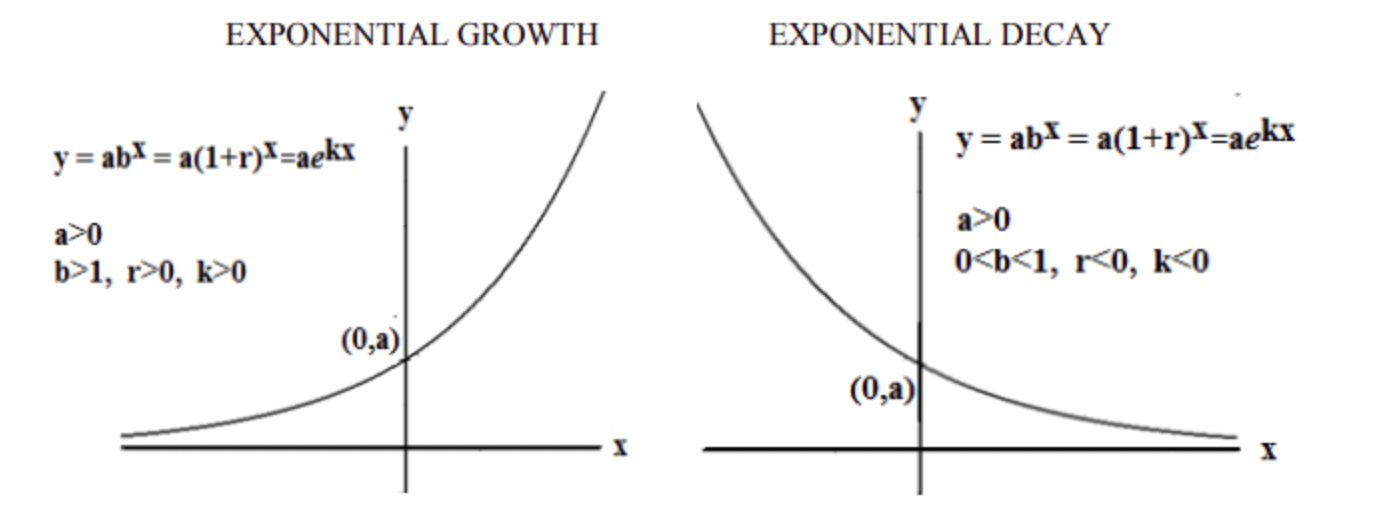
\includegraphics[width=15cm]{ExponentialGrowthandDecay.png}
\caption{Exponential Growth and Exponential Decay}
\label{exp}
\end{figure}



\end{itemize}

\section{Functional Requirement}
\subsection{Definitions and abbreviations}
\begin{center}
    \begin{tabular}{|c|c|}
         \hline
         Term & Definition \\
         \hline\hline
         FR & Functional Requirement \\
         \hline
         NFR & Non-Functional Requirement \\
         \hline
         User & End user are the human users who interacts with the system \\
         \hline
         System & Application which is used for solving exponential function. \\
         \hline
        \end{tabular}
        \label{tab:xyz}
         \captionof{table}{Definitions and abbreviations}
\end{center}

\subsection{Assumptions}
\begin{itemize}
    \item The calculator must accepts the exponential constant like e in addition to the constants a and b.
    \item

\end{itemize}

\subsection{Requirements}



\subsubsection{Functional Requirements}
\begin{itemize}
    \item
    \textbf{ID } \hspace{3cm} :FR1  \\
	\textbf{Type } \hspace{2.4cm}  :Functional\\
	\textbf{Version Number} \hspace{0.3cm} :1.0  \\
	\textbf{Owner } \hspace{1.98cm} : Avneet \\
	\textbf{Priority } \hspace{1.75cm} : High\\
	\textbf{Difficulty } \hspace{1.5cm} : Easy \\
	\textbf{Description }\hspace{1.2cm} :The calculator should ask the user to input a, b, and x. \\
	\textbf{Rationale }\hspace{1.6cm} :In order to process function f(x) = a$b^x$ and give output system needs input form the user. \\

	\item
    \textbf{ID } \hspace{3cm} :FR2  \\
	\textbf{Type } \hspace{2.4cm}  :Functional\\
	\textbf{Version Number} \hspace{0.3cm} :1.0  \\
	\textbf{Owner } \hspace{1.98cm} : Avneet \\
	\textbf{Priority } \hspace{1.75cm} : High\\
	\textbf{Difficulty } \hspace{1.5cm} : Easy\\
	\textbf{Description }\hspace{1.2cm} :When a user input is not a number, the system should provide an error message. \\
	\textbf{Rationale }\hspace{1.6cm} :The only acceptable input for an exponential function calculation is a number. \\

	\item
    \textbf{ID } \hspace{3cm} :FR3  \\
	\textbf{Type } \hspace{2.4cm}  :Functional\\
	\textbf{Version Number} \hspace{0.3cm} :1.0  \\
	\textbf{Owner } \hspace{1.98cm} : Avneet \\
	\textbf{Priority } \hspace{1.75cm} : High\\
	\textbf{Difficulty } \hspace{1.5cm} : Easy\\
	\textbf{Description }\hspace{1.2cm} :If a user enters incorrect data, the system shouldn't shut down but rather prompt users to reenter their data.\\
	\textbf{Rationale }\hspace{1.6cm} :The ability to perform calculations again and without closing the programme should be available to the user. \\

	\item
    \textbf{ID } \hspace{3cm} :FR4  \\
	\textbf{Type } \hspace{2.4cm}  :Functional\\
	\textbf{Version Number} \hspace{0.3cm} :1.0  \\
	\textbf{Owner } \hspace{1.98cm} : Avneet \\
	\textbf{Priority } \hspace{1.75cm} : High\\
	\textbf{Difficulty } \hspace{1.5cm} : Easy\\
	\textbf{Description }\hspace{1.2cm} : Whole numbers and rational numbers are accepted as user inputs.\\
	\textbf{Rationale }\hspace{1.6cm} : The code does not handle irrational numbers. For instance, $\pi$, $\sqrt{2}$ \\

	\item
    \textbf{ID } \hspace{3cm} :FR5  \\
	\textbf{Type } \hspace{2.4cm}  :Functional\\
	\textbf{Version Number} \hspace{0.3cm} :1.0  \\
	\textbf{Owner } \hspace{1.98cm} : Avneet \\
	\textbf{Priority } \hspace{1.75cm} : High\\
	\textbf{Difficulty } \hspace{1.5cm} : Easy\\
	\textbf{Description }\hspace{1.2cm} : Fractional inputs must be entered as double values.\\
	\textbf{Rationale }\hspace{1.6cm} : If a user wants to provide a base or exponent value of 1/2, they must do so as 0.5.\\

	\item
    \textbf{ID } \hspace{3cm} :FR6  \\
	\textbf{Type } \hspace{2.4cm}  :Functional\\
	\textbf{Version Number} \hspace{0.3cm} :1.0  \\
	\textbf{Owner } \hspace{1.98cm} : Avneet \\
	\textbf{Priority } \hspace{1.75cm} : High\\
	\textbf{Difficulty } \hspace{1.5cm} : Easy\\
	\textbf{Description }\hspace{1.2cm} : Base b is restricted to positive number.\\
	\textbf{Rationale }\hspace{1.6cm} : In order to guarantee $b^x$ is real number.\\


	\item
    \textbf{ID } \hspace{3cm} :FR7  \\
	\textbf{Type } \hspace{2.4cm}  :Functional\\
	\textbf{Version Number} \hspace{0.3cm} :1.0  \\
	\textbf{Owner } \hspace{1.98cm} : Avneet \\
	\textbf{Priority } \hspace{1.75cm} : High\\
	\textbf{Difficulty } \hspace{1.5cm} : Easy\\
	\textbf{Description }\hspace{1.2cm} : When any base value of b is raised to the power of x=0, the function's $b^x$ portion must return the value 1.\\
	\textbf{Rationale }\hspace{1.6cm} : For instance: 11 raised to the power 0 gives 1.\\

	\item
    \textbf{ID } \hspace{3cm} :FR8  \\
	\textbf{Type } \hspace{2.4cm}  :Functional\\
	\textbf{Version Number} \hspace{0.3cm} :1.0  \\
	\textbf{Owner } \hspace{1.98cm} : Avneet \\
	\textbf{Priority } \hspace{1.75cm} : High\\
	\textbf{Difficulty } \hspace{1.5cm} : Easy\\
	\textbf{Description }\hspace{1.2cm} : When base value b=0 is raised to any exponent value, the $b^x$ portion of the function must return 0.\\
	\textbf{Rationale }\hspace{1.6cm} : For instance, 0 raised to the power 11 yields 0.\\

\end{itemize}
\subsubsection{Non-Functional Requirements}
\begin{itemize}

	\item
    \textbf{ID } \hspace{3cm} :NFR1  \\
	\textbf{Type } \hspace{2.4cm}  :Non-Functional\\
	\textbf{Version Number} \hspace{0.3cm} :1.0  \\
	\textbf{Owner } \hspace{1.98cm} : Avneet \\
	\textbf{Priority } \hspace{1.75cm} : High\\
	\textbf{Difficulty } \hspace{1.5cm} : Easy\\
	\textbf{Description }\hspace{1.2cm} :An error message should be informative and relevant to the user.\\
	\textbf{Rationale }\hspace{1.6cm} : The user should be able to resolve simple problems on their own by understanding error message to enhance usability.\\

	\item
    \textbf{ID } \hspace{3cm} :NFR2  \\
	\textbf{Type } \hspace{2.4cm}  :Non-Functional\\
	\textbf{Version Number} \hspace{0.3cm} :1.0  \\
	\textbf{Owner } \hspace{1.98cm} : Avneet \\
	\textbf{Priority } \hspace{1.75cm} : High\\
	\textbf{Difficulty } \hspace{1.5cm} : Easy\\
	\textbf{Description }\hspace{1.2cm} :The command line interface ought to be user-friendly.\\
	\textbf{Rationale }\hspace{1.6cm} : The system should be simple for the user to operate. \\

	\item
    \textbf{ID } \hspace{3cm} :NFR3  \\
	\textbf{Type } \hspace{2.4cm}  :Non-Functional\\
	\textbf{Version Number} \hspace{0.3cm} :1.0  \\
	\textbf{Owner } \hspace{1.98cm} : Avneet \\
	\textbf{Priority } \hspace{1.75cm} : High\\
	\textbf{Difficulty } \hspace{1.5cm} : Easy\\
	\textbf{Description }\hspace{1.2cm} :The outcome must be accurate.\\
	\textbf{Rationale }\hspace{1.6cm} :  To enhance the accuracy of system. It is inappropriate to display incorrect ouptut to the user.\\

	\item
    \textbf{ID } \hspace{3cm} :NFR4  \\
	\textbf{Type } \hspace{2.4cm}  :Non-Functional\\
	\textbf{Version Number} \hspace{0.3cm} :1.0  \\
	\textbf{Owner } \hspace{1.98cm} : Avneet \\
	\textbf{Priority } \hspace{1.75cm} : High\\
	\textbf{Difficulty } \hspace{1.5cm} : Easy\\
	\textbf{Description }\hspace{1.2cm} :There should be no more than 5 seconds of calculation time.\\
	\textbf{Rationale }\hspace{1.6cm} :  In order to improve the performance of the system.\\

	\item
    \textbf{ID } \hspace{3cm} :NFR5  \\
	\textbf{Type } \hspace{2.4cm}  :Non-Functional\\
	\textbf{Version Number} \hspace{0.3cm} :1.0  \\
	\textbf{Owner } \hspace{1.98cm} : Avneet \\
	\textbf{Priority } \hspace{1.75cm} : High\\
	\textbf{Difficulty } \hspace{1.5cm} : Easy\\
	\textbf{Description }\hspace{1.2cm} : System should be maintainable for the duration of its anticipated lifetime and able to accommodate new requirements in response to stakeholders' changing needs. \\
	\textbf{Rationale }\hspace{1.6cm} : Since future changes to software systems are inevitable. Maintainable systems are therefore simpler to alter.\\

	\item
    \textbf{ID } \hspace{3cm} :NFR6  \\
	\textbf{Type } \hspace{2.4cm}  :Non-Functional\\
	\textbf{Version Number} \hspace{0.3cm} :1.0  \\
	\textbf{Owner } \hspace{1.98cm} : Avneet \\
	\textbf{Priority } \hspace{1.75cm} : High\\
	\textbf{Difficulty } \hspace{1.5cm} : Easy\\
	\textbf{Description }\hspace{1.2cm} : The system should be developed using widely used and standardised language. \\
	\textbf{Rationale }\hspace{1.6cm} : Java is used to build a system which is platform independent hence make the system portable.\\


\end{itemize}

\section{Algorithm}

\subsection{Pseudocode}

\begin{algorithm}
\caption{Iterative Algorithm to calculate: $ab^x$ }
\begin{algorithmic}
\Procedure{$calculateExponentialFunction$}{$a,b,x$}
\State \textbf{input: } String a, b, x
\State \textbf{output: } double res
\State  res = 1
\State temp = 1
\If{((a $||$ b) == "0")}
    \Return res
\Else
    \If{(b == "e")}
        \State res = exponentialFunc(x,n)
    \State end
\State \Return a * res
    \Else
        \State for temp $<=$x
            \State res = res * b
            \State temp = temp + 1
        \State end
        \State \Return a*res
        \EndIf
\EndIf
\EndProcedure

\\
\Procedure{$exponentialFunc$}{$x, n$}
\State \textbf{input: } int x, int n
\State \textbf{output: } double res
\State power = 1
\State factorial = 1
\State recursive
\If{(n==0)}
    \State \Return 1
\EndIf
\State recursive = exponentialFunc(x, n-1)
\State power = power * x
\State factorial = factorial * n
\State \Return (recursive + power/factorial)
\EndProcedure
\\

\end{algorithmic}
\end{algorithm}

% Second logic: recursive approach
\begin{algorithm}
\caption{Recursive Algorithm to calculate: $ab^x$ }
\begin{algorithmic}
\Procedure{$calculateExponentialFunction$}{$a,b,x$}
\State \textbf{input: } string a, b, x
\State \textbf{output: } double res
\State  res=0
\If{(a $||$ b == 0)}
    \State \Return res
\ElsIf{(b=="e")}
    \State res = naturalExponential(x)
\Else
 \State res = calculatePower(b,x)
\EndIf
\State res = $a * res$
\State \Return res
\EndProcedure
\\
\Procedure{$naturalExponential$}{$x$}
\State \textbf{input: } int x
\State \textbf{output: } double exposum
\State nterms = 25
\State exposum = 1
\State for i $<=$ nterms
    \State exposum = 1+x * exposum/i
    \State end
\State \Return exposum
\EndProcedure
\\
\Procedure{$calculatePower$}{$b,x$}
\State \textbf{input: } double b, int x
\State \textbf{output: } double res
\If{(($x < 0$)}
\State \Return $1.0/powHelper(b,x)$
   \EndIf
\State \Return $powHelper(b,x)$
\EndProcedure
\\
\Procedure{$powHelper$}{$b,x$}
\State \textbf{input: } double b, int x
\State \textbf{output: } double res
\If{($x == 0$)}
    \Return 1
\EndIf
\If{($x == 1$)}
    \Return b
\EndIf
\If{($x mod 2$ == 0)}
\State \Return $powerHandler(b*b,  n/2)$
\Else
\State \Return $b * powerHandler(b*b,  n/2)$
\EndIf
\EndProcedure
\end{algorithmic}
% \end{algorithm}

\end{algorithm}

\pagebreak

\subsection{Description}

\subsubsection{Algorithm1}

\textbf{ Description: }
\begin{itemize}
    \item \textbf{Case 1:} When base has been assigned with any number, then for  loop will keep multiplying result variable by base variable until the power becomes zero. And then result is multiplied with constant a.
    \item \textbf{Case 2:} When base has been assigned with natural exponential constant “e”. Then the function is computed using Taylor series. Since Taylor Series is a combination of multiple values like sum, power and factorial term, hence we will use static variables.
\end{itemize}

\textbf{ Rationale: } Due to its $O(n^2)$ time complexity and linear space constraints in calculating exponential function and O(n) for power calculations, this algorithm was discarded.So, in the following algorithm 2 I tried to make it efficient.
\\\textbf{ Complexity: } $O(n)$, $O(n^2)$
\\\textbf{ Advantages: }
\begin{enumerate}
    \item In iterative solution, there is no stack overflow exception where stack can take no more frames.
    \item Iterative algorithms are easy to understand and readable by human.

\end{enumerate}
\textbf{ Disadvantages: }
\begin{enumerate}
    \item For case 1, this algorithm is taking O(n) time complexity.
    \item For case 2, this algorithm is taking $O(n^2)$ time complexity and O(n) Space complexity.

\end{enumerate}


\subsubsection{Algorithm2}

\textbf{ Description: }
\begin{itemize}
    \item \textbf{Case 1:}When base is assigned any numeric value, calculatePower() function is called which in further calls powerhandler() function to consider cases where power is negative and positive.
    \item \textbf{Case 2:}When base has been assigned with natural exponential constant “e”, we calculated the sum using for loop, and calculated it for n terms using Taylor Series.
\end{itemize}
\textbf{ Rationale: } In Algorithm 1 case 1 is optimized to $O(log n)$ and case 2 is optimized to  O(n). So the decision of implementing Algorithm 2 is made since its more time and space efficient.
\\\textbf{ Complexity: } $O(log n)$, O(n)
\\\textbf{ Advantages: }
\begin{enumerate}
    \item Recursion add clarity to the code and reduce time while debugging code.
    \item In this we tried to avoid stack overflow exception by handling all possible edge cases efficiently.
\end{enumerate}
\textbf{ Disadvantages: }
\begin{enumerate}
    \item Recursive methods will often throw a StackOverflowException when processing big numeric values.

\end{enumerate}

\subsection{Mindmap for Pseudocode format Selection}

\section{Debugger, Quality Attributes, Checkstyle}
\subsection{Debugger}
\subsubsection{Description}A debugger is a tool that can be used to examine what is happening in a programme. This allows you to find bugs by carefully analysing how the programme is executed. One can examine the behaviour of code using a debugger without changing the source code.

\textbf{Debugger Used:} Used inbuilt debugger provided by IntelliJ IDEA.

\subsubsection{Advantages}
\begin{enumerate}
    \item \textbf{Saves Time:} Debugger helps developer in identifying erroneous state of program. For example, if ode is breaking somewhere, then debugger comes to rescue to identify the root cause of error and hence saves time of developer.
    \item \textbf{Bug free end product: } Debugger allows early fault detection and hence give enough time to developers to fix the error and release bug free software to customers.
    \item \textbf{Watchpoints: } To edit code without restarting your program, Watchpoints comes to rescue and helps in inspecting data items or other objects.
\end{enumerate}
\subsubsection{Disadvantages}
\begin{enumerate}
    \item The downside of Debugger is that developers cannot debug microservices easily and serverless application in local environment.
    \item Debugging remotely is also difficult since its dependent on permission, which require access and admin privileges to the server.
\end{enumerate}
\subsubsection{Snapshots}

\begin{figure}
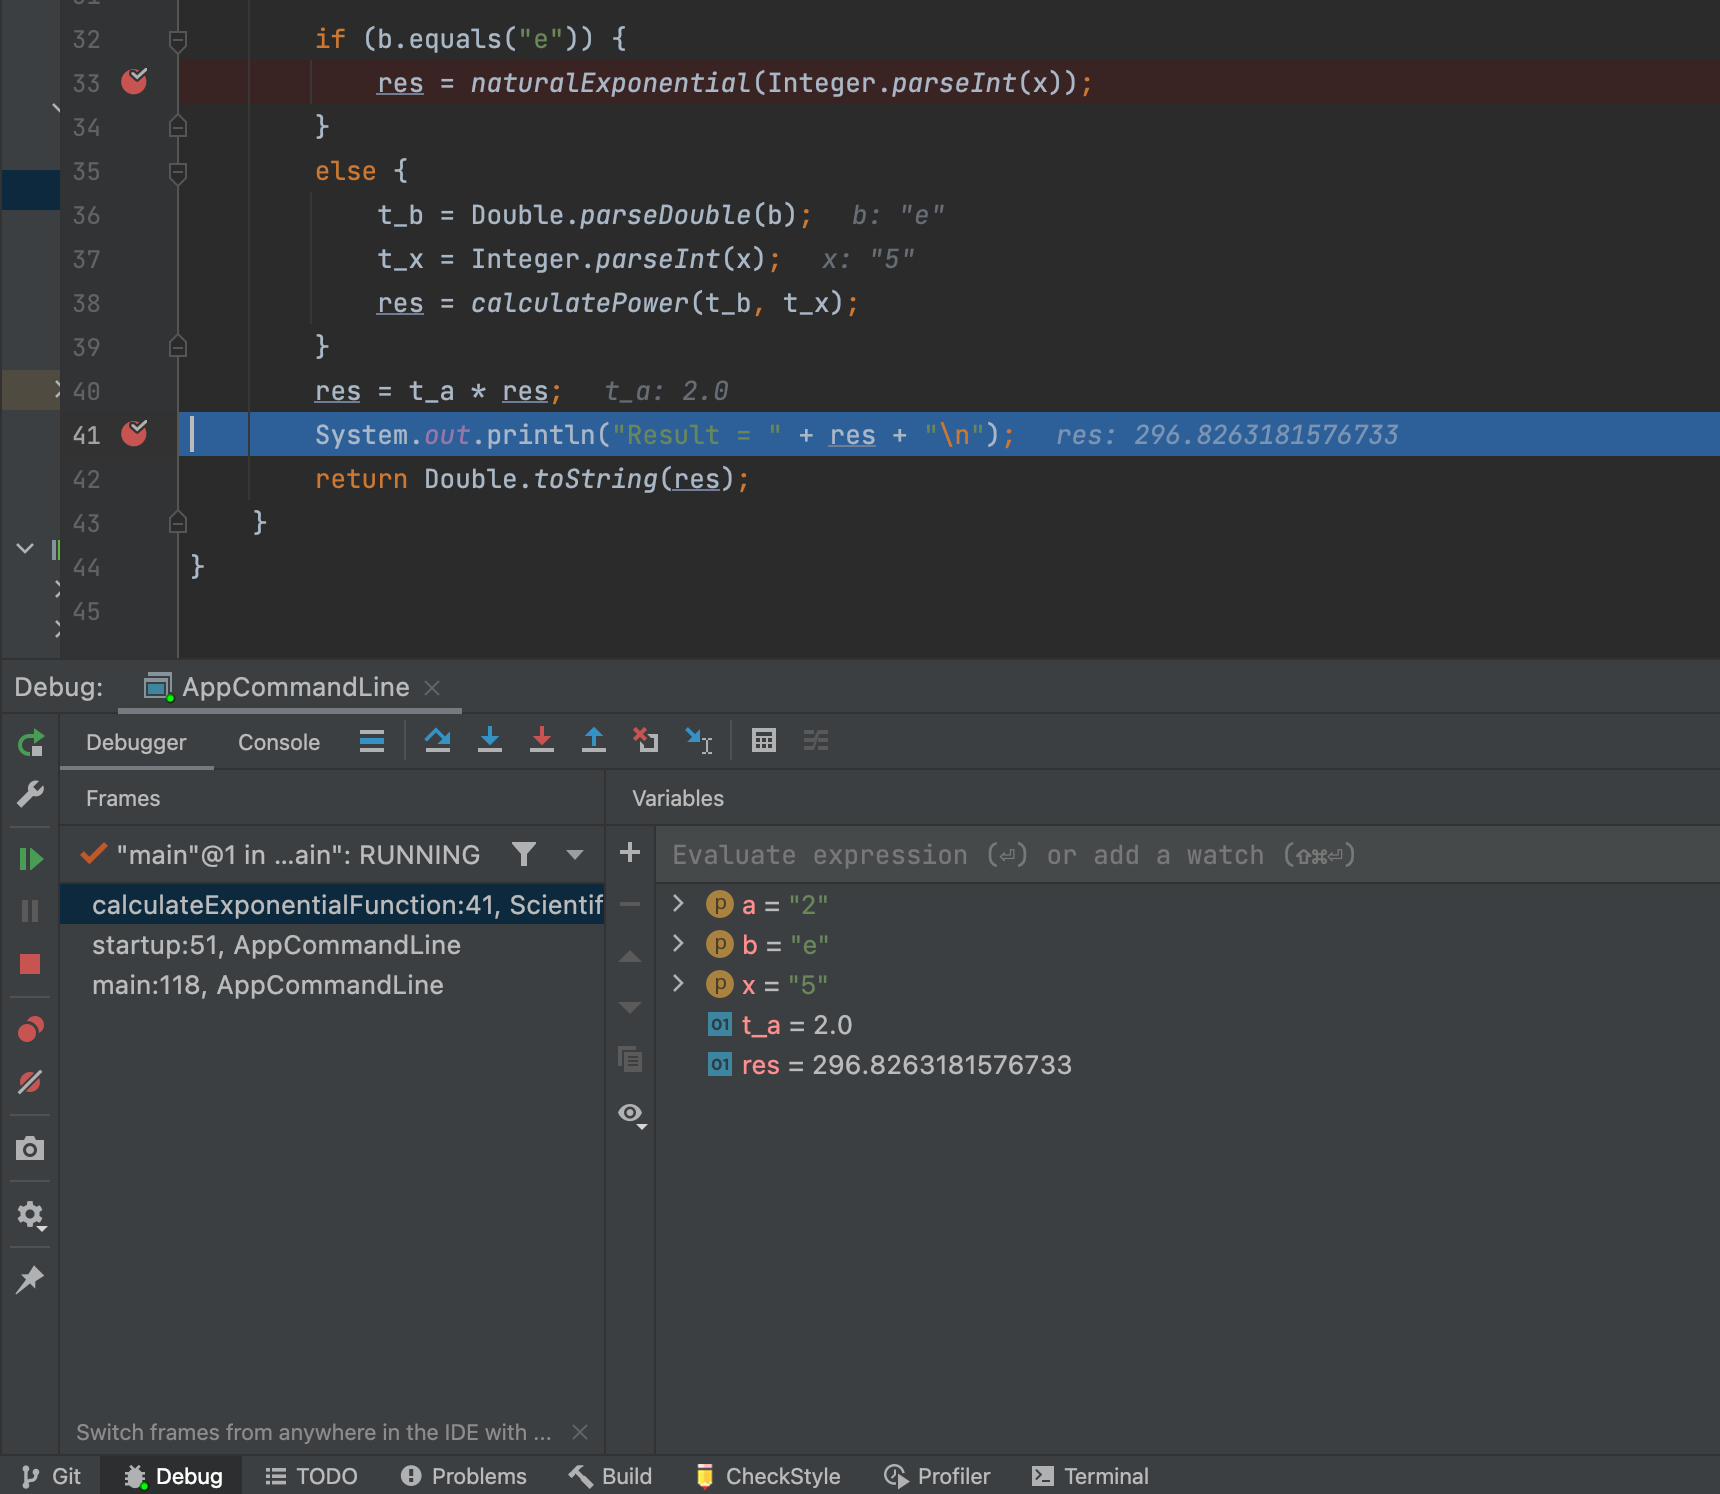
\includegraphics[width=15cm]{LineBreakpoint.png}
\caption{Snapshot representing usage of Line Breakpoint while debugging}
\label{exp}
\end{figure}

\begin{figure}
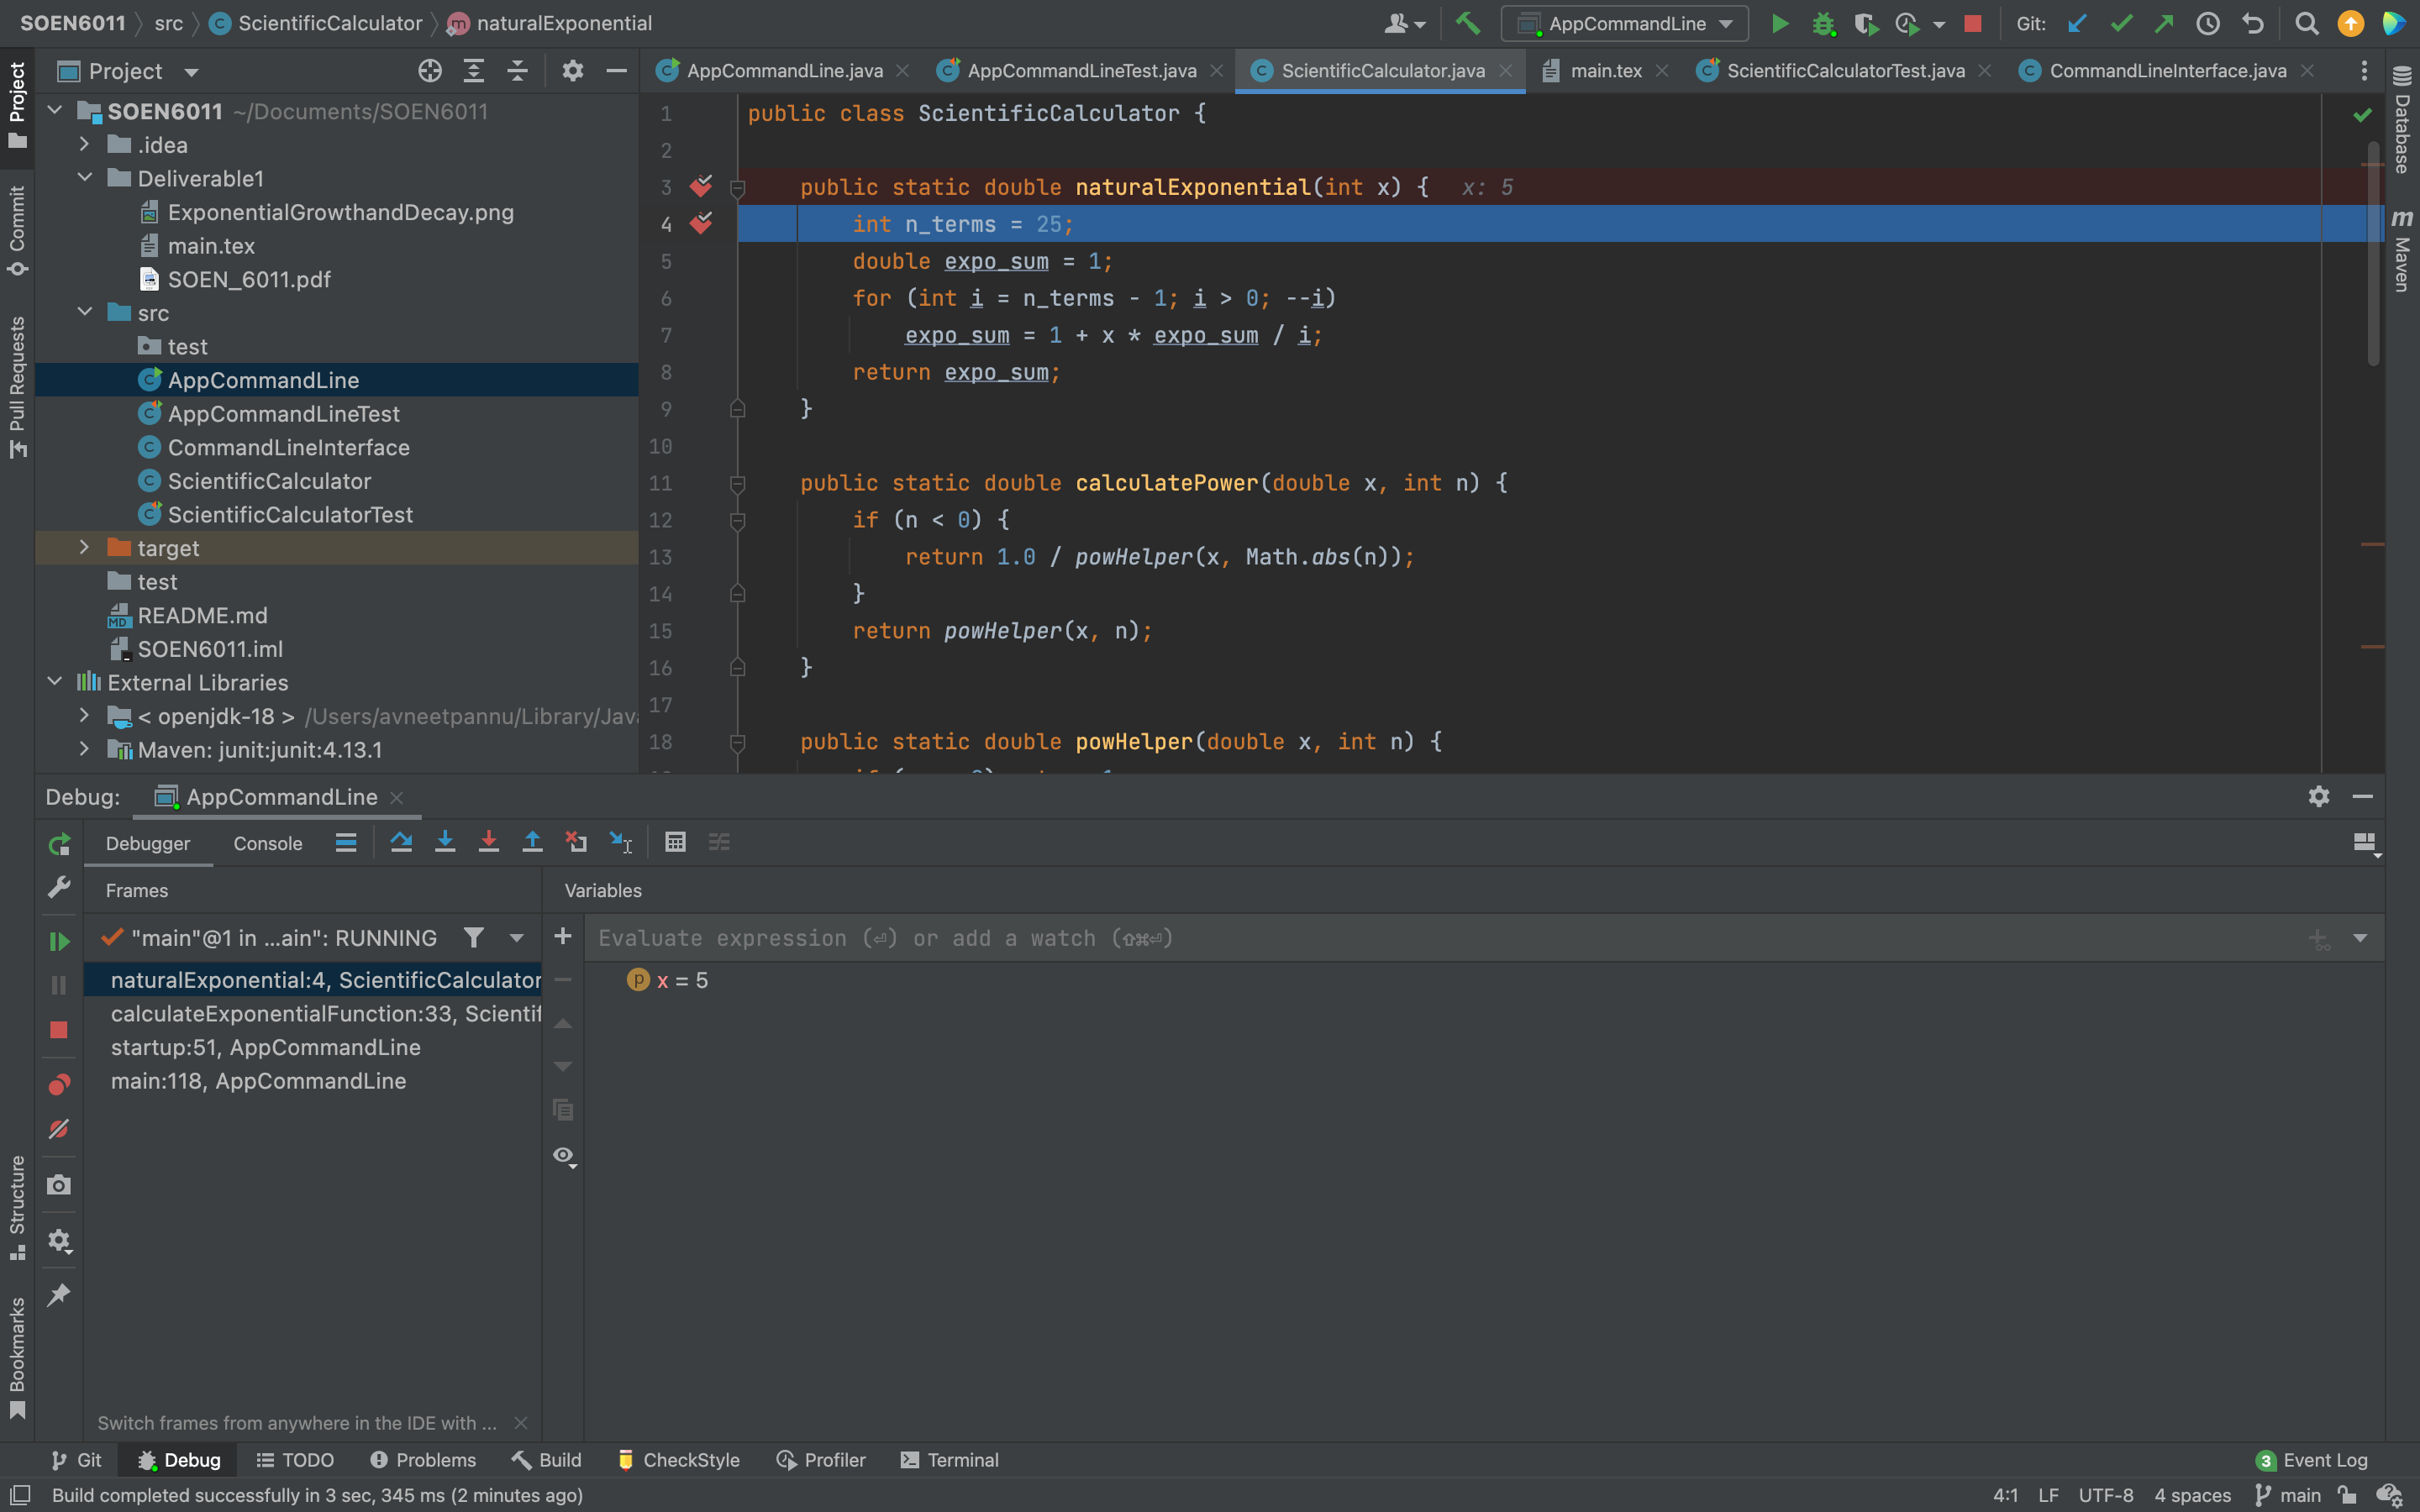
\includegraphics[width=15cm]{MethodBreakpoint.png}
\caption{Snapshot representing usage of Method Breakpoint}
\label{exp}
\end{figure}

\pagebreak

\subsection{Quality Attributes}
\subsubsection{Robustness}
\begin{enumerate}
   \item Each time new functionality was released, a corresponding Unit case was developed and tested.
   \item Included all potential edge cases for the calculating function.
   \item Handled all the potential exceptions properly.
\end{enumerate}
\subsubsection{Maintainability}
\begin{enumerate}
   \item Each method that has been defined has been properly commented.
   \item Global variables should not be used to ensure future maintenance.
   \item Refactoring code in accordance with coding standards after each commit to a github branch.
\end{enumerate}
\subsubsection{Correctness}
\begin{enumerate}
   \item Adhering to java coding standards.
   \item To check the correctness of all the functionality, JUnit test cases are implemented.
   \item Displaying correct result while on successful calculation..
\end{enumerate}
\subsubsection{Usability}
\begin{enumerate}
   \item A command-line interface that is easy to use.
    \item Showing a menu of the functions a calculator can perform.
    \item Providing customers with a helpful error message that tries to assist them in identifying minor mistakes

\end{enumerate}


\pagebreak
\subsection{Checkstyle}
\subsubsection{Description} To help programmers to adhere Java coding standard and to check the pragmatic quality of Java Code, development tool known as Checkstyle is used. It helps in checking Java code automatically. Also, developers can define there own set of rules and check code against their rules.
\\\textbf{Checkstyle Used:} Used Sun Code Conventions checkstyle provided by Checkstyle-IDEA.


\subsubsection{Advantages}
\begin{enumerate}
    \item Helps in resolving Class and method design problems.
    \item Helps in resolving formatting issues.
\end{enumerate}
\subsubsection{Disadvantages}
\begin{enumerate}
    \item Configuration is time consuming, it needs external plugins to download.
    \item To configure checkstyle, some people prefer making changes to maven configuration which is also error-prone and takes time to resolve.
\end{enumerate}
\subsubsection{Snapshots}
\pagebreak
\begin{figure}
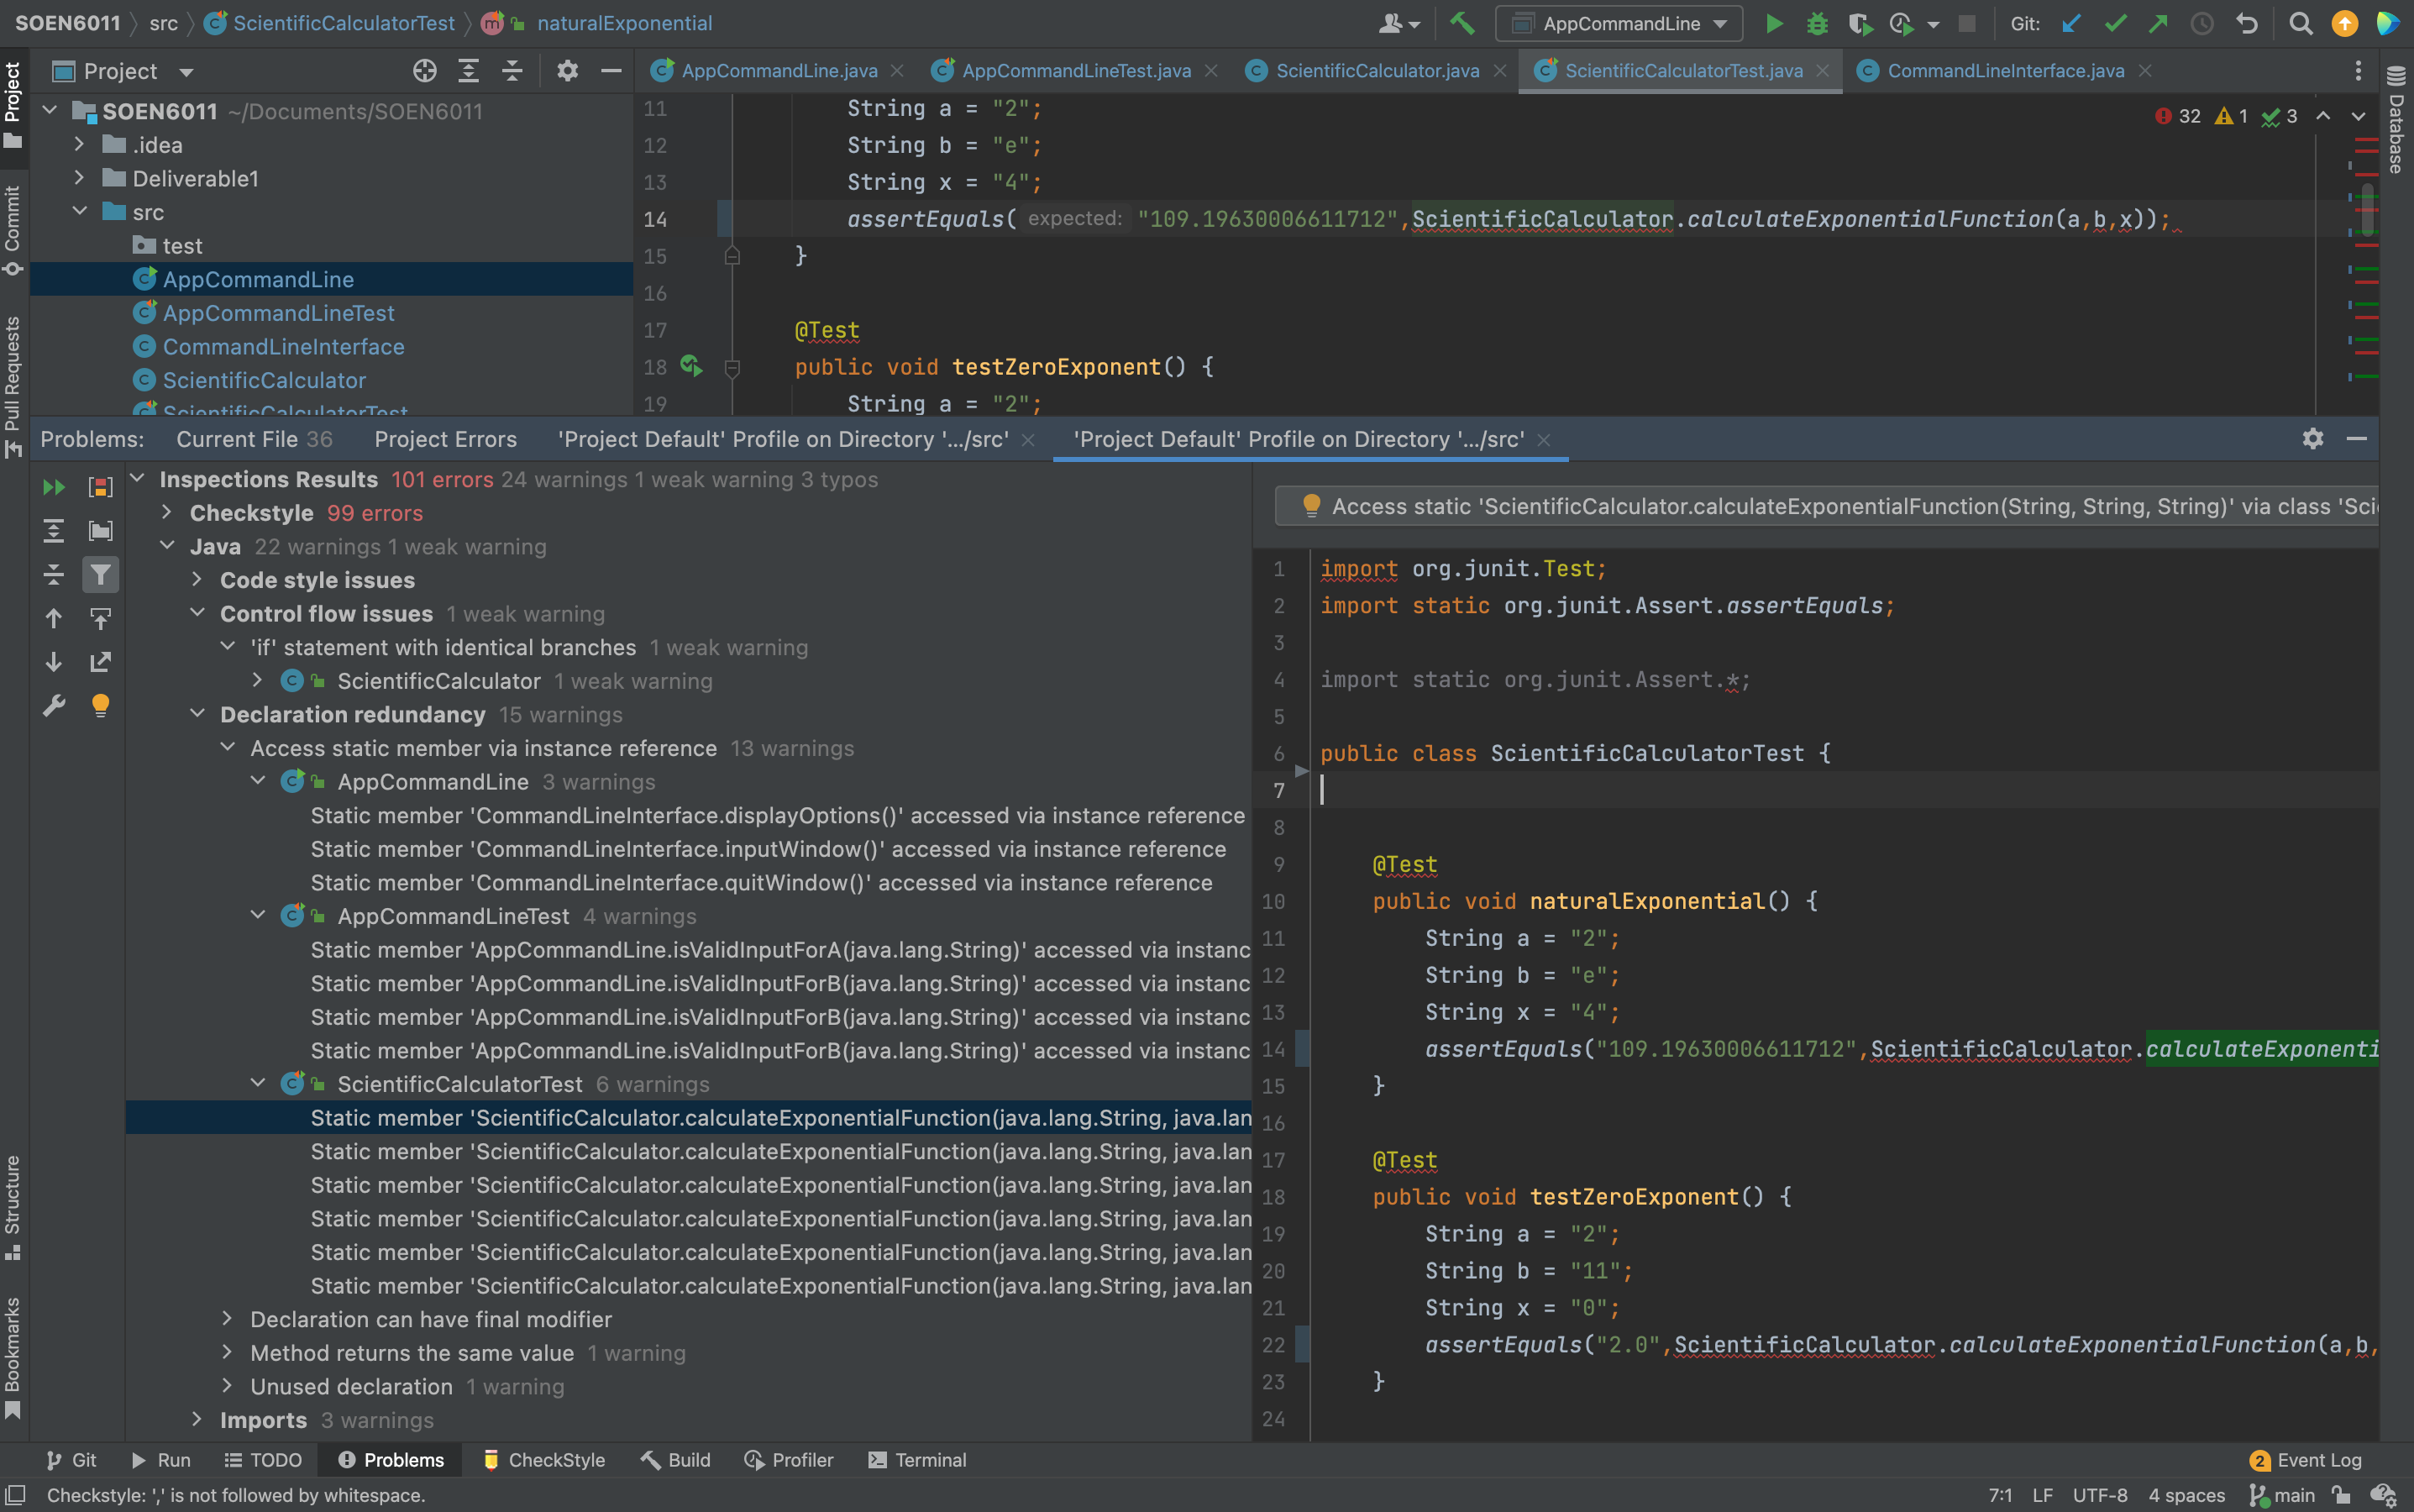
\includegraphics[width=15cm]{Checkstyle.png}
\caption{Snapshot representing the usage of checkstyle}
\label{exp}
\end{figure}


\section{Unit Tests}
\subsection{Standard Guidelines}
\subsection{Traceability}






\begin{thebibliography}{9}
\bibitem{b1} Zill, D. G., \& Wright, W. S. (2011). Calculus: Early transcendentals. Jones and Bartlett Publishers.
\bibitem{b2} Rock, N. M. (2007). Standards driven math. student standards handbook. Team Rock Press.
\bibitem{b3}Exponential growth and decay - virtuallearningacademy.net. (n.d.). Retrieved August 3, 2022, from  \url{https://virtuallearningacademy.net/VLA/LessonDisplay/Lesson6156/MATHALGIIBU17Exponential_Decay.pdf}
\bibitem{b4}GeeksforGeeks. (2022, July 19). Write a program to calculate POW(X,N). GeeksforGeeks. Retrieved August 5, 2022, from https://www.geeksforgeeks.org/write-a-c-program-to-calculate-powxn/
\bibitem{b5}Exponential Function Calculator. High accuracy calculation for life or science. (n.d.). Retrieved August 5, 2022, from https://keisan.casio.com/exec/system/1223447896
\end{thebibliography}
\end{document}
